\label {fs-dataflow}

Typical classification pipeline based on bag-of-words text representation consists of three steps. The first one is computing TF-IDF features. The second one is training a classifier on these features or making a prediction. To adapt this pipeline for a stream processing engine, one needs to represent it in the form of a {\em logical graph}. It serves as a descriptive language for defining streaming computations. Vertices of a logical graph denote operations, while edges indicate data subscriptions between them. 

The initial point in our data flow is an {\em Source} vertex. It receives input texts from data producers and computes term frequencies. Computing of inverse document frequencies is a separate operation because it maintains a state and requires different data partitioning in a physical execution that we touch upon further. {\em TF-IDF} vertex joins features corresponding to the same text and passes them to the {\em Text Classifier}. {\em Text Classifier} is the very last vertex that predicts a label and delivers it to a data consumer. The scheme of the proposed logical graph is shown in Figure~\ref{logical_graph}.

\begin{figure}[htbp]
  \centering
  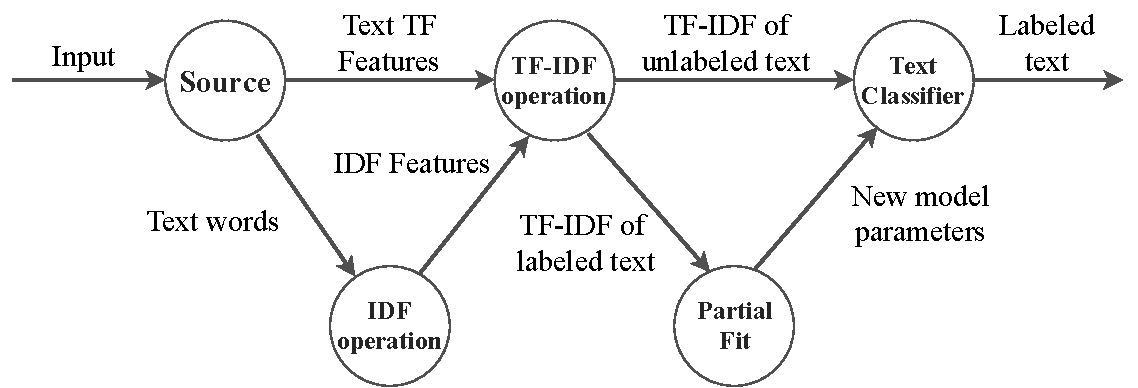
\includegraphics[scale=0.38]{pics/logical-graph}
  \caption{Text classification data flow}
  \label {logical_graph}
\end{figure}

Training pipeline is a separate branch within the logical graph introduced above. For already labeled text its features are sent to a {\em Partial fit} vertex instead of the {\em Classifier}. {\em Partial fit} vertex buffers all input elements until training is triggered. After training, the buffer flushes. Updated parameters of a machine learning model are saved for further training and broadcasted to all {\em Text Classifier} vertices.